\documentclass{beamer}

\usepackage{préambule}

\begin{document}

\begin{frame}
	{\small Écrire l'énoncé !}
	\begin{enumerate}
		\item Construire une droite, et placer un point $O$ vers le milieu, et un point $I$ à sa droite. On considérera maintenant que l'abscisse de $O$ est $0$, et l'abscisse de $I$ est $1$.
		\item Placer les nombres suivants sur la droite, \textbf{en utilisant uniquement une règle non graduée et un compas} :
		      \begin{enumerate}[a.]
			      \item $2$
			      \item $-1$
			      \item $-2$
			      \item $\dfrac{1}{2}$
			      \item $\sqrt{2}$
		      \end{enumerate}
	\end{enumerate}


\end{frame}

\newcommand{\placePoint}[3]{
	\draw[#3] (#1, 0) -- ++(0,-0.2) node[below] {#2};
}

\begin{frame}
	\begin{center}
		\begin{tikzpicture}
			\draw[\myArrow] (-5.5,0) -- (5.5,0);
			\placePoint{0}{$O$}{}
			\placePoint{2}{$I$}{}

			\pause

			\placePoint{4}{$2$}{red}
			\placePoint{-2}{$-1$}{red}
			\placePoint{-4}{$-2$}{red}
			\placePoint{1}{$\dfrac{1}{2}$}{red}
			\placePoint{2.8284271247461903}{$\sqrt{2}$}{red}
		\end{tikzpicture}
	\end{center}
\end{frame}


\begin{frame}
	Quel nombre peut-on placer avec la figure suivante ?
	\begin{center}
		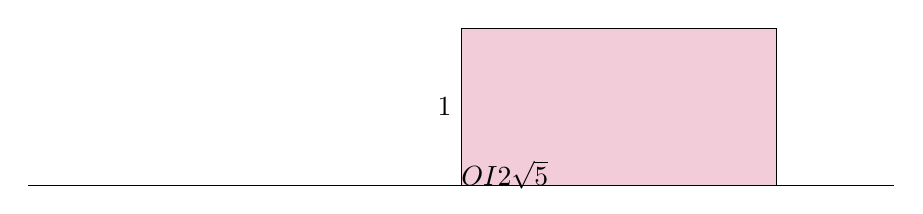
\begin{tikzpicture}
			\draw[fill=purple!20] (0,0) -- ++(4,0) -- ++(0,2) -- ++(-4,0) -- node[midway,left] {$1$} cycle;
			\draw[\myArrow] (-5.5,0) -- (5.5,0);
			\placePoint{0}{$O$}{}
			\placePoint{2}{$I$}{}
			\placePoint{4}{$2$}{}


			\pause

			\placePoint{4.47213595499958}{$\sqrt{5}$}{red}
		\end{tikzpicture}
	\end{center}
\end{frame}

\end{document}